% ============================================================
% 讲义 — 人教版高二选择性必修第二册 第5章
% 一元函数的导数及其应用
% 编译命令：xelatex -interaction=nonstopmode 文件名.tex
% ============================================================
\documentclass[12pt, a4paper]{ctexart}
\usepackage[margin=2.2cm]{geometry}
\usepackage{amsmath, amssymb}
\usepackage{enumitem}
\usepackage{tcolorbox}
\usepackage{booktabs}
\usepackage{array}
\usepackage{fancyhdr}
\usepackage{xcolor}
\usepackage{tikz}
\usepackage{hyperref}
\usepackage{graphicx}
\usepackage{multirow}
\usepackage{pgfplots}
\pgfplotsset{compat=1.18}

% 颜色定义
\definecolor{mainblue}{RGB}{41, 98, 168}
\definecolor{lightblue}{RGB}{230, 240, 255}
\definecolor{tipgreen}{RGB}{34, 139, 87}
\definecolor{lightgreen}{RGB}{235, 250, 240}
\definecolor{warnred}{RGB}{200, 50, 50}
\definecolor{lightred}{RGB}{255, 240, 240}
\definecolor{examorange}{RGB}{210, 120, 20}
\definecolor{lightorange}{RGB}{255, 248, 235}
\definecolor{apppurple}{RGB}{120, 60, 170}
\definecolor{lightpurple}{RGB}{245, 238, 255}

% 页眉页脚
\pagestyle{fancy}
\fancyhf{}
\fancyhead[L]{\small\textcolor{mainblue}{\textbf{人教版高二选必2 · 第5章 一元函数的导数及其应用}}}
\fancyhead[R]{\small\textcolor{mainblue}{导数及其应用讲义}}
\fancyfoot[C]{\small —\ \thepage\ —}
\renewcommand{\headrulewidth}{0.6pt}
\renewcommand{\headrule}{\hbox to\headwidth{\color{mainblue}\leaders\hrule height \headrulewidth\hfill}}
\renewcommand{\footrulewidth}{0pt}

% tcolorbox 样式
\newtcolorbox{knowledgebox}[1][]{%
  colback=lightblue, colframe=mainblue,
  fonttitle=\bfseries\large, title=#1,
  arc=3mm, boxrule=0.8pt,
  left=8pt, right=8pt, top=6pt, bottom=6pt
}

\newtcolorbox{tipbox}[1][]{%
  colback=lightgreen, colframe=tipgreen,
  fonttitle=\bfseries, title=#1,
  arc=2mm, boxrule=0.6pt,
  left=6pt, right=6pt, top=4pt, bottom=4pt
}

\newtcolorbox{warnbox}[1][]{%
  colback=lightred, colframe=warnred,
  fonttitle=\bfseries, title=#1,
  arc=2mm, boxrule=0.6pt,
  left=6pt, right=6pt, top=4pt, bottom=4pt
}

\newtcolorbox{examplebox}[1][]{%
  colback=lightorange, colframe=examorange,
  fonttitle=\bfseries, title=#1,
  arc=3mm, boxrule=0.8pt,
  left=8pt, right=8pt, top=6pt, bottom=6pt
}

\newtcolorbox{appbox}[1][]{%
  colback=lightpurple, colframe=apppurple,
  fonttitle=\bfseries, title=#1,
  arc=3mm, boxrule=0.8pt,
  left=8pt, right=8pt, top=6pt, bottom=6pt
}

\setCJKmainfont{Hiragino Sans GB}
\setCJKsansfont{Heiti SC}

\begin{document}

% ============ 标题页 ============
\begin{center}
{\Huge\bfseries\textcolor{mainblue}{第5章\quad 一元函数的导数及其应用}}\\[12pt]
{\Large\textcolor{gray}{讲\quad 义}}\\[8pt]
\rule{0.6\textwidth}{1pt}\\[8pt]
{\normalsize 适用：人教版\quad 高二选择性必修第二册\quad |\quad 课时：5课时}
\end{center}
\vspace{10pt}

% ============================================================
% 第一部分：知识点讲解
% ============================================================
\section*{\textcolor{mainblue}{一、知识点讲解}}

% ===== 5.1 导数的概念 =====
\subsection*{5.1\quad 导数的概念与几何意义}

\begin{knowledgebox}[导数的定义]
设函数 $y = f(x)$ 在点 $x_0$ 的某邻域内有定义，当自变量 $x$ 在 $x_0$ 处取得增量 $\Delta x$（点 $x_0 + \Delta x$ 仍在该邻域内）时，相应的函数取得增量 $\Delta y = f(x_0 + \Delta x) - f(x_0)$。如果 $\Delta y$ 与 $\Delta x$ 之比当 $\Delta x \to 0$ 时的极限存在，则称函数 $y = f(x)$ 在点 $x_0$ 处\textbf{可导}，并称此极限值为函数 $y = f(x)$ 在点 $x_0$ 处的\textbf{导数}，记作 $f'(x_0)$，即
\[
f'(x_0) = \lim_{\Delta x \to 0} \frac{\Delta y}{\Delta x} = \lim_{\Delta x \to 0} \frac{f(x_0 + \Delta x) - f(x_0)}{\Delta x}
\]
\end{knowledgebox}

\begin{knowledgebox}[导数的几何意义]
函数 $y = f(x)$ 在点 $x_0$ 处的导数 $f'(x_0)$ 的几何意义是：曲线 $y = f(x)$ 在点 $(x_0, f(x_0))$ 处的\textbf{切线斜率}。

由此可得曲线在点 $(x_0, f(x_0))$ 处的：
\begin{itemize}[leftmargin=2em]
  \item \textbf{切线方程}：$y - f(x_0) = f'(x_0)(x - x_0)$
  \item \textbf{法线方程}：$y - f(x_0) = -\dfrac{1}{f'(x_0)}(x - x_0)$\quad（$f'(x_0) \neq 0$ 时）
\end{itemize}
\end{knowledgebox}

\begin{warnbox}[易错提醒]
\begin{enumerate}[leftmargin=2em]
  \item 导数存在 $\Leftrightarrow$ 左导数 $=$ 右导数，即 $f'_-(x_0) = f'_+(x_0)$。
  \item 可导一定连续，但连续不一定可导（如 $y = |x|$ 在 $x=0$ 处连续但不可导）。
  \item 求切线方程时，要先确认所给点是否在曲线上。若点不在曲线上，需先设切点坐标。
\end{enumerate}
\end{warnbox}

% ===== 5.2 基本初等函数的导数公式 =====
\subsection*{5.2\quad 基本初等函数的导数公式}

\begin{knowledgebox}[基本导数公式表]
\begin{center}
\renewcommand{\arraystretch}{1.6}
\begin{tabular}{>{\centering\arraybackslash}p{5cm} >{\centering\arraybackslash}p{7cm}}
\toprule
\textbf{原函数 $f(x)$} & \textbf{导数 $f'(x)$} \\
\midrule
$C$（常数） & $0$ \\
$x^n$（$n$ 为常数） & $nx^{n-1}$ \\
$\sin x$ & $\cos x$ \\
$\cos x$ & $-\sin x$ \\
$\tan x$ & $\sec^2 x = \dfrac{1}{\cos^2 x}$ \\
$a^x$（$a > 0, a \neq 1$） & $a^x \ln a$ \\
$e^x$ & $e^x$ \\
$\log_a x$（$a > 0, a \neq 1$） & $\dfrac{1}{x \ln a}$ \\
$\ln x$ & $\dfrac{1}{x}$ \\
$\sqrt{x}$ & $\dfrac{1}{2\sqrt{x}}$ \\
\bottomrule
\end{tabular}
\end{center}
\end{knowledgebox}

\begin{tipbox}[记忆技巧]
\begin{itemize}[leftmargin=2em]
  \item 三角函数求导：\textbf{正变余，余变负}。$(\sin x)' = \cos x$，$(\cos x)' = -\sin x$。
  \item 指数函数：以 $e$ 为底的指数函数求导不变，即 $(e^x)' = e^x$。
  \item 对数函数：自然对数最简洁，$(\ln x)' = \frac{1}{x}$。
  \item 幂函数：指数下来，指数减1，即 $(x^n)' = nx^{n-1}$。
\end{itemize}
\end{tipbox}

% ===== 5.3 导数的运算法则 =====
\subsection*{5.3\quad 导数的运算法则}

\begin{knowledgebox}[导数的四则运算法则]
设 $u = u(x)$，$v = v(x)$ 均可导，则：
\begin{enumerate}[leftmargin=2em]
  \item \textbf{和差法则}：$(u \pm v)' = u' \pm v'$
  \item \textbf{积法则}：$(uv)' = u'v + uv'$
  \item \textbf{商法则}：$\left(\dfrac{u}{v}\right)' = \dfrac{u'v - uv'}{v^2}$\quad（$v \neq 0$）
\end{enumerate}
\end{knowledgebox}

\begin{warnbox}[易错提醒]
\begin{itemize}[leftmargin=2em]
  \item $(uv)' \neq u'v'$，不要误将乘积的导数写成导数的乘积。
  \item $\left(\dfrac{u}{v}\right)' \neq \dfrac{u'}{v'}$，商法则的分子是"下乘上导减上乘下导"。
  \item 特别地，$(Cu)' = Cu'$（$C$ 为常数），常数因子可以直接提出来。
\end{itemize}
\end{warnbox}

% ===== 5.4 复合函数求导 =====
\subsection*{5.4\quad 复合函数的求导法则（链式法则）}

\begin{knowledgebox}[链式法则]
如果 $y = f(u)$，$u = g(x)$ 都可导，则复合函数 $y = f(g(x))$ 的导数为：
\[
\frac{dy}{dx} = \frac{dy}{du} \cdot \frac{du}{dx} = f'(u) \cdot g'(x) = f'(g(x)) \cdot g'(x)
\]
即：\textbf{外层对内层求导 $\times$ 内层对自变量求导}。
\end{knowledgebox}

\begin{tipbox}[复合函数求导步骤]
\begin{enumerate}[leftmargin=2em]
  \item \textbf{分层}：将复合函数分解为外层函数和内层函数。
  \item \textbf{逐层求导}：先对外层求导（内层保持不变），再乘以内层对自变量的导数。
  \item \textbf{回代}：将内层函数代回，使最终结果只含自变量 $x$。
\end{enumerate}
\end{tipbox}

\begin{warnbox}[常见复合函数求导示例]
\begin{itemize}[leftmargin=2em]
  \item $y = \sin(2x + 1)$：$y' = \cos(2x+1) \cdot 2 = 2\cos(2x+1)$
  \item $y = e^{3x}$：$y' = e^{3x} \cdot 3 = 3e^{3x}$
  \item $y = (x^2 + 1)^5$：$y' = 5(x^2+1)^4 \cdot 2x = 10x(x^2+1)^4$
  \item $y = \ln(3x - 2)$：$y' = \dfrac{1}{3x-2} \cdot 3 = \dfrac{3}{3x-2}$
  \item $y = \sqrt{x^2 + 4}$：$y' = \dfrac{1}{2\sqrt{x^2+4}} \cdot 2x = \dfrac{x}{\sqrt{x^2+4}}$
\end{itemize}
\end{warnbox}

% ===== 5.5 导数与函数的单调性 =====
\subsection*{5.5\quad 导数与函数的单调性}

\begin{knowledgebox}[导数与单调性的关系]
设函数 $f(x)$ 在区间 $(a, b)$ 内可导：
\begin{enumerate}[leftmargin=2em]
  \item 若 $f'(x) > 0$ 在 $(a, b)$ 内恒成立，则 $f(x)$ 在 $(a, b)$ 上\textbf{单调递增}。
  \item 若 $f'(x) < 0$ 在 $(a, b)$ 内恒成立，则 $f(x)$ 在 $(a, b)$ 上\textbf{单调递减}。
  \item 若 $f'(x) = 0$ 在 $(a, b)$ 内恒成立，则 $f(x)$ 在 $(a, b)$ 上为\textbf{常数函数}。
\end{enumerate}
\end{knowledgebox}

\begin{knowledgebox}[求函数单调区间的步骤]
\begin{enumerate}[leftmargin=2em]
  \item 求函数 $f(x)$ 的定义域。
  \item 求导数 $f'(x)$。
  \item 令 $f'(x) = 0$，求出所有实数根（驻点）。
  \item 用驻点将定义域划分为若干区间。
  \item 在每个区间内判断 $f'(x)$ 的符号，从而确定单调性。
\end{enumerate}
\end{knowledgebox}

\begin{tipbox}[方法总结]
\begin{itemize}[leftmargin=2em]
  \item $f'(x) > 0$ 是 $f(x)$ 单调递增的\textbf{充分不必要}条件。例如 $f(x) = x^3$ 在 $x = 0$ 处 $f'(0) = 0$，但 $f(x)$ 在 $\mathbb{R}$ 上单调递增。
  \item 单调性是"区间"上的性质，不能说在某一点处单调。
  \item 若 $f'(x)$ 在某区间内恒大于等于零（等于零的点为孤立点），则函数仍单调递增。
\end{itemize}
\end{tipbox}

% ===== 5.6 导数与函数的极值、最值 =====
\subsection*{5.6\quad 导数与函数的极值、最值}

\begin{knowledgebox}[极值的定义与判定]
\textbf{极值}：若 $f(x_0)$ 是函数 $f(x)$ 在 $x_0$ 附近（某邻域内）的最大值（或最小值），则称 $f(x_0)$ 为 $f(x)$ 的\textbf{极大值}（或\textbf{极小值}），$x_0$ 称为\textbf{极大值点}（或\textbf{极小值点}）。

\textbf{极值的必要条件}（费马定理）：若 $f(x)$ 在 $x_0$ 处可导且取得极值，则 $f'(x_0) = 0$。

\textbf{极值的第一充分条件}：设 $f(x)$ 在 $x_0$ 处连续，在 $x_0$ 的某去心邻域内可导：
\begin{itemize}[leftmargin=2em]
  \item 若 $x < x_0$ 时 $f'(x) > 0$，$x > x_0$ 时 $f'(x) < 0$，则 $f(x_0)$ 为\textbf{极大值}。
  \item 若 $x < x_0$ 时 $f'(x) < 0$，$x > x_0$ 时 $f'(x) > 0$，则 $f(x_0)$ 为\textbf{极小值}。
\end{itemize}
\end{knowledgebox}

\begin{knowledgebox}[求函数极值的步骤]
\begin{enumerate}[leftmargin=2em]
  \item 求导数 $f'(x)$。
  \item 令 $f'(x) = 0$，解方程求驻点。
  \item 检查每个驻点两侧 $f'(x)$ 的符号变化，判断极大值或极小值。
  \item 代入原函数求出极值。
\end{enumerate}
\end{knowledgebox}

\begin{knowledgebox}[闭区间上函数的最值]
求 $f(x)$ 在 $[a, b]$ 上的最大值和最小值的步骤：
\begin{enumerate}[leftmargin=2em]
  \item 求 $f(x)$ 在 $(a, b)$ 内所有使 $f'(x) = 0$ 的点的函数值。
  \item 求端点函数值 $f(a)$ 和 $f(b)$。
  \item 比较以上所有函数值，\textbf{最大的为最大值，最小的为最小值}。
\end{enumerate}
\end{knowledgebox}

\begin{warnbox}[易错提醒]
\begin{itemize}[leftmargin=2em]
  \item 极值是\textbf{局部}概念，最值是\textbf{整体}概念。极值不一定是最值，最值不一定是极值（最值可能在端点取到）。
  \item $f'(x_0) = 0$ 只是极值的必要条件，不是充分条件。例如 $f(x) = x^3$，$f'(0) = 0$，但 $x = 0$ 不是极值点。
  \item 不可导的点也可能是极值点，如 $f(x) = |x|$ 在 $x = 0$ 处。
\end{itemize}
\end{warnbox}

% ============================================================
% 第二部分：例题精讲
% ============================================================
\section*{\textcolor{examorange}{二、例题精讲}}

% ----- 例题1：导数定义 -----
\begin{examplebox}[【例题1】利用导数定义求导数]
已知 $f(x) = x^2 - 3x + 1$，利用导数定义求 $f'(2)$。
\end{examplebox}

\textbf{解}：由导数定义：
\begin{align*}
f'(2) &= \lim_{\Delta x \to 0} \frac{f(2 + \Delta x) - f(2)}{\Delta x} \\
&= \lim_{\Delta x \to 0} \frac{[(2+\Delta x)^2 - 3(2+\Delta x) + 1] - [4 - 6 + 1]}{\Delta x} \\
&= \lim_{\Delta x \to 0} \frac{4 + 4\Delta x + (\Delta x)^2 - 6 - 3\Delta x + 1 + 1}{\Delta x} \\
&= \lim_{\Delta x \to 0} \frac{(\Delta x)^2 + \Delta x}{\Delta x} \\
&= \lim_{\Delta x \to 0} (\Delta x + 1) = 1
\end{align*}

\begin{tipbox}[方法总结]
用导数定义求 $f'(x_0)$ 的关键是计算极限 $\displaystyle\lim_{\Delta x \to 0} \frac{f(x_0 + \Delta x) - f(x_0)}{\Delta x}$。先化简分式，约去 $\Delta x$，再取极限。
\end{tipbox}

% ----- 例题2：求切线方程 -----
\begin{examplebox}[【例题2】求曲线的切线方程]
求曲线 $y = x^3 - 2x + 1$ 在点 $(1, 0)$ 处的切线方程。
\end{examplebox}

\textbf{解}：
\begin{enumerate}[leftmargin=2em]
  \item 验证：$f(1) = 1 - 2 + 1 = 0$，点 $(1, 0)$ 在曲线上。
  \item 求导：$f'(x) = 3x^2 - 2$。
  \item 切线斜率：$k = f'(1) = 3(1)^2 - 2 = 1$。
  \item 切线方程：$y - 0 = 1 \cdot (x - 1)$，即 $y = x - 1$。
\end{enumerate}

\begin{center}
\begin{tikzpicture}
\begin{axis}[
  width=10cm, height=7cm,
  axis lines=middle,
  xlabel=$x$, ylabel=$y$,
  xmin=-2, xmax=3, ymin=-4, ymax=6,
  grid=both,
  grid style={dotted, gray!40},
  legend pos=north west,
  samples=100,
]
\addplot[mainblue, thick, domain=-1.8:2.5]{x^3 - 2*x + 1};
\addlegendentry{$y = x^3 - 2x + 1$}
\addplot[warnred, thick, domain=-0.5:2.5]{x - 1};
\addlegendentry{$y = x - 1$（切线）}
\addplot[only marks, mark=*, mark size=2.5pt, black] coordinates {(1, 0)};
\node[anchor=south west] at (axis cs:1.1, 0.1) {$(1, 0)$};
\end{axis}
\end{tikzpicture}
\end{center}

% ----- 例题3：复合函数求导 -----
\begin{examplebox}[【例题3】复合函数求导]
求下列函数的导数：
\begin{enumerate}[leftmargin=2em]
  \item $y = e^{2x} \sin 3x$
  \item $y = \dfrac{\ln x}{x^2 + 1}$
  \item $y = (2x - 1)^4$
\end{enumerate}
\end{examplebox}

\textbf{解}：

(1) 由积法则和链式法则：
\begin{align*}
y' &= (e^{2x})' \sin 3x + e^{2x} (\sin 3x)' \\
&= 2e^{2x} \sin 3x + e^{2x} \cdot 3\cos 3x \\
&= e^{2x}(2\sin 3x + 3\cos 3x)
\end{align*}

(2) 由商法则：
\begin{align*}
y' &= \frac{(\ln x)'(x^2 + 1) - \ln x \cdot (x^2 + 1)'}{(x^2 + 1)^2} \\
&= \frac{\dfrac{1}{x}(x^2 + 1) - \ln x \cdot 2x}{(x^2 + 1)^2} \\
&= \frac{x^2 + 1 - 2x^2 \ln x}{x(x^2 + 1)^2}
\end{align*}

(3) 由链式法则：令 $u = 2x - 1$，则 $y = u^4$。
\[
y' = 4u^3 \cdot u' = 4(2x-1)^3 \cdot 2 = 8(2x-1)^3
\]

% ----- 例题4：判断单调性 -----
\begin{examplebox}[【例题4】判断函数的单调性]
讨论函数 $f(x) = x^3 - 3x + 1$ 的单调性，并求其单调区间。
\end{examplebox}

\textbf{解}：
\begin{enumerate}[leftmargin=2em]
  \item $f(x)$ 的定义域为 $\mathbb{R}$。
  \item $f'(x) = 3x^2 - 3 = 3(x + 1)(x - 1)$。
  \item 令 $f'(x) = 0$，得 $x = -1$ 或 $x = 1$。
  \item 列表讨论：
\end{enumerate}

\begin{center}
\renewcommand{\arraystretch}{1.4}
\begin{tabular}{c|c|c|c}
\toprule
$x$ & $(-\infty, -1)$ & $(-1, 1)$ & $(1, +\infty)$ \\
\midrule
$f'(x)$ & $+$ & $-$ & $+$ \\
$f(x)$ & $\nearrow$ & $\searrow$ & $\nearrow$ \\
\bottomrule
\end{tabular}
\end{center}

因此，$f(x)$ 在 $(-\infty, -1)$ 和 $(1, +\infty)$ 上单调递增，在 $(-1, 1)$ 上单调递减。

\begin{center}
\begin{tikzpicture}
\begin{axis}[
  width=10cm, height=7cm,
  axis lines=middle,
  xlabel=$x$, ylabel=$y$,
  xmin=-3.5, xmax=3.5, ymin=-4, ymax=5,
  grid=both,
  grid style={dotted, gray!40},
  samples=200,
]
\addplot[mainblue, thick, domain=-2.5:2.5]{x^3 - 3*x + 1};
\addlegendentry{$y = x^3 - 3x + 1$}
\addplot[only marks, mark=*, mark size=2.5pt, warnred] coordinates {(-1, 3)};
\addplot[only marks, mark=*, mark size=2.5pt, warnred] coordinates {(1, -1)};
\node[anchor=south] at (axis cs:-1, 3.4) {$(-1, 3)$（极大值）};
\node[anchor=north] at (axis cs:1, -1.4) {$(1, -1)$（极小值）};
\end{axis}
\end{tikzpicture}
\end{center}

% ----- 例题5：求极值 -----
\begin{examplebox}[【例题5】求函数的极值]
求函数 $f(x) = 2x^3 - 6x^2 + 7$ 的极值。
\end{examplebox}

\textbf{解}：
\begin{enumerate}[leftmargin=2em]
  \item $f'(x) = 6x^2 - 12x = 6x(x - 2)$。
  \item 令 $f'(x) = 0$，得 $x = 0$ 或 $x = 2$。
  \item 列表讨论：
\end{enumerate}

\begin{center}
\renewcommand{\arraystretch}{1.4}
\begin{tabular}{c|c|c|c}
\toprule
$x$ & $(-\infty, 0)$ & $(0, 2)$ & $(2, +\infty)$ \\
\midrule
$f'(x)$ & $+$ & $-$ & $+$ \\
$f(x)$ & $\nearrow$ & $\searrow$ & $\nearrow$ \\
\bottomrule
\end{tabular}
\end{center}

\begin{itemize}[leftmargin=2em]
  \item $x = 0$：$f'(x)$ 由正变负，$f(0) = 7$ 为\textbf{极大值}。
  \item $x = 2$：$f'(x)$ 由负变正，$f(2) = 16 - 24 + 7 = -1$ 为\textbf{极小值}。
\end{itemize}

\begin{center}
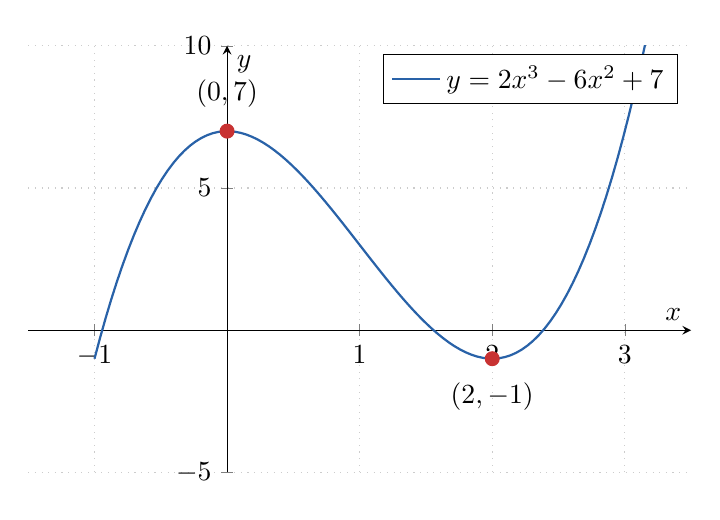
\begin{tikzpicture}
\begin{axis}[
  width=10cm, height=7cm,
  axis lines=middle,
  xlabel=$x$, ylabel=$y$,
  xmin=-1.5, xmax=3.5, ymin=-5, ymax=10,
  grid=both,
  grid style={dotted, gray!40},
  samples=100,
]
\addplot[mainblue, thick, domain=-1:3.2]{2*x^3 - 6*x^2 + 7};
\addlegendentry{$y = 2x^3 - 6x^2 + 7$}
\addplot[only marks, mark=*, mark size=2.5pt, warnred] coordinates {(0, 7)};
\addplot[only marks, mark=*, mark size=2.5pt, warnred] coordinates {(2, -1)};
\node[anchor=south] at (axis cs:0, 7.5) {$(0, 7)$};
\node[anchor=north] at (axis cs:2, -1.5) {$(2, -1)$};
\end{axis}
\end{tikzpicture}
\end{center}

% ----- 例题6：含参单调性讨论 -----
\begin{examplebox}[【例题6】含参函数的单调性讨论]
已知函数 $f(x) = x^3 + ax^2 + bx + 1$，在 $x = -1$ 处取得极大值，在 $x = 3$ 处取得极小值。求 $a$、$b$ 的值。
\end{examplebox}

\textbf{解}：$f'(x) = 3x^2 + 2ax + b$。

由题意，$x = -1$ 和 $x = 3$ 是 $f'(x) = 0$ 的两个根，因此：
\begin{align*}
f'(-1) &= 3 - 2a + b = 0 \\
f'(3) &= 27 + 6a + b = 0
\end{align*}

两式相减：$24 + 8a = 0$，解得 $a = -3$。

代入第一式：$3 + 6 + b = 0$，解得 $b = -9$。

\textbf{验证}：$f'(x) = 3x^2 - 6x - 9 = 3(x+1)(x-3)$。
\begin{itemize}[leftmargin=2em]
  \item $x < -1$ 时 $f'(x) > 0$，$-1 < x < 3$ 时 $f'(x) < 0$，故 $x = -1$ 为极大值点。
  \item $-1 < x < 3$ 时 $f'(x) < 0$，$x > 3$ 时 $f'(x) > 0$，故 $x = 3$ 为极小值点。
\end{itemize}
符合题意，因此 $a = -3$，$b = -9$。

% ----- 例题7：闭区间最值 -----
\begin{examplebox}[【例题7】闭区间上求最值]
求函数 $f(x) = x^3 - 3x^2 + 1$ 在 $[-1, 4]$ 上的最大值和最小值。
\end{examplebox}

\textbf{解}：
\begin{enumerate}[leftmargin=2em]
  \item $f'(x) = 3x^2 - 6x = 3x(x - 2)$。
  \item 令 $f'(x) = 0$，得 $x = 0$ 或 $x = 2$，均在 $[-1, 4]$ 内。
  \item 计算各关键点的函数值：
\end{enumerate}
\begin{align*}
f(-1) &= -1 - 3 + 1 = -3 \\
f(0) &= 0 - 0 + 1 = 1 \\
f(2) &= 8 - 12 + 1 = -3 \\
f(4) &= 64 - 48 + 1 = 17
\end{align*}

比较得：\textbf{最大值为 $f(4) = 17$，最小值为 $f(-1) = f(2) = -3$}。

% ----- 例题8：过曲线外一点求切线 -----
\begin{examplebox}[【例题8】过曲线外一点的切线方程]
过点 $(0, -2)$ 作曲线 $y = x^3 - 3x$ 的切线，求切线方程。
\end{examplebox}

\textbf{解}：设切点为 $(t, t^3 - 3t)$。

$y' = 3x^2 - 3$，切线斜率 $k = 3t^2 - 3$。

切线方程：$y - (t^3 - 3t) = (3t^2 - 3)(x - t)$。

切线过点 $(0, -2)$，代入得：
\[
-2 - (t^3 - 3t) = (3t^2 - 3)(0 - t)
\]
\[
-2 - t^3 + 3t = -3t^3 + 3t
\]
\[
-2 - t^3 + 3t + 3t^3 - 3t = 0
\]
\[
2t^3 = 2 \implies t^3 = 1 \implies t = 1
\]

切点为 $(1, -2)$，斜率 $k = 3(1)^2 - 3 = 0$。

切线方程为 $y = -2$。

\begin{center}
\begin{tikzpicture}
\begin{axis}[
  width=10cm, height=7cm,
  axis lines=middle,
  xlabel=$x$, ylabel=$y$,
  xmin=-3, xmax=3, ymin=-5, ymax=5,
  grid=both,
  grid style={dotted, gray!40},
  samples=100,
]
\addplot[mainblue, thick, domain=-2.2:2.2]{x^3 - 3*x};
\addlegendentry{$y = x^3 - 3x$}
\addplot[warnred, thick, domain=-3:3]{-2};
\addlegendentry{$y = -2$（切线）}
\addplot[only marks, mark=*, mark size=2.5pt, black] coordinates {(1, -2)};
\addplot[only marks, mark=square*, mark size=2.5pt, examorange] coordinates {(0, -2)};
\node[anchor=south east] at (axis cs:1, -2) {切点 $(1, -2)$};
\node[anchor=north west] at (axis cs:0, -2) {$(0, -2)$};
\end{axis}
\end{tikzpicture}
\end{center}

% ----- 例题9：导数与不等式 -----
\begin{examplebox}[【例题9】利用导数证明不等式]
证明：当 $x > 0$ 时，$e^x > 1 + x$。
\end{examplebox}

\textbf{证明}：令 $f(x) = e^x - 1 - x$（$x > 0$）。

$f'(x) = e^x - 1$。

当 $x > 0$ 时，$e^x > 1$，故 $f'(x) > 0$。

因此 $f(x)$ 在 $(0, +\infty)$ 上单调递增。

又 $f(0) = e^0 - 1 - 0 = 0$。

所以当 $x > 0$ 时，$f(x) > f(0) = 0$，即 $e^x - 1 - x > 0$。

故 $e^x > 1 + x$。\quad $\square$

\begin{tipbox}[方法总结]
利用导数证明不等式的一般步骤：
\begin{enumerate}[leftmargin=2em]
  \item 构造辅助函数 $f(x)$（将不等式移项使一边为 $0$）。
  \item 利用导数分析 $f(x)$ 的单调性。
  \item 利用单调性和某个已知点的函数值，得出不等式。
\end{enumerate}
\end{tipbox}

% ----- 例题10：综合应用 -----
\begin{examplebox}[【例题10】含参讨论极值个数]
已知函数 $f(x) = x^3 - 3ax + 1$（$a$ 为常数），讨论 $f(x)$ 的极值个数。
\end{examplebox}

\textbf{解}：$f'(x) = 3x^2 - 3a = 3(x^2 - a)$。

\textbf{情形一}：$a \leqslant 0$ 时，$f'(x) = 3(x^2 - a) \geqslant 0$ 恒成立（当 $a = 0$ 时仅在 $x = 0$ 处取等号）。

$f(x)$ 在 $\mathbb{R}$ 上单调递增，\textbf{无极值}。

\textbf{情形二}：$a > 0$ 时，令 $f'(x) = 0$，得 $x = -\sqrt{a}$ 或 $x = \sqrt{a}$。

\begin{center}
\renewcommand{\arraystretch}{1.4}
\begin{tabular}{c|c|c|c}
\toprule
$x$ & $(-\infty, -\sqrt{a})$ & $(-\sqrt{a}, \sqrt{a})$ & $(\sqrt{a}, +\infty)$ \\
\midrule
$f'(x)$ & $+$ & $-$ & $+$ \\
$f(x)$ & $\nearrow$ & $\searrow$ & $\nearrow$ \\
\bottomrule
\end{tabular}
\end{center}

$f(x)$ 在 $x = -\sqrt{a}$ 处取得极大值，在 $x = \sqrt{a}$ 处取得极小值，\textbf{有两个极值}。

\textbf{综上}：当 $a \leqslant 0$ 时，$f(x)$ 无极值；当 $a > 0$ 时，$f(x)$ 有极大值和极小值共两个极值。

% ----- 例题11：构造函数求参数 -----
\begin{examplebox}[【例题11】利用单调性求参数范围]
已知函数 $f(x) = x^3 + ax$ 在 $\mathbb{R}$ 上单调递增，求实数 $a$ 的取值范围。
\end{examplebox}

\textbf{解}：$f'(x) = 3x^2 + a$。

$f(x)$ 在 $\mathbb{R}$ 上单调递增 $\Leftrightarrow$ $f'(x) \geqslant 0$ 对一切 $x \in \mathbb{R}$ 恒成立。

即 $3x^2 + a \geqslant 0$ 对一切 $x \in \mathbb{R}$ 恒成立。

由于 $3x^2 \geqslant 0$，故 $a \geqslant -3x^2$ 对一切 $x$ 成立。

而 $-3x^2$ 的最大值为 $0$（当 $x = 0$ 时），故 $a \geqslant 0$。

因此 $a$ 的取值范围为 $\boxed{a \geqslant 0}$。

% ============================================================
% 第三部分：应用题
% ============================================================
\section*{\textcolor{apppurple}{三、应用题}}

% ----- 应用1：最优化问题 -----
\begin{appbox}[【应用1】用料最省问题]
一个开口的圆柱形容器，容积为 $V = 2\pi \text{ m}^3$。问底面半径 $r$ 为多少时，所用材料（即表面积）最省？
\end{appbox}

\textbf{解}：设底面半径为 $r$（m），高为 $h$（m）。

由容积 $V = \pi r^2 h = 2\pi$，得 $h = \dfrac{2}{r^2}$。

表面积（开口容器）：
\[
S = \pi r^2 + 2\pi r h = \pi r^2 + 2\pi r \cdot \frac{2}{r^2} = \pi r^2 + \frac{4\pi}{r} \quad (r > 0)
\]

求导：
\[
S'(r) = 2\pi r - \frac{4\pi}{r^2} = \frac{2\pi(r^3 - 2)}{r^2}
\]

令 $S'(r) = 0$，得 $r^3 = 2$，即 $r = \sqrt[3]{2}$。

当 $0 < r < \sqrt[3]{2}$ 时，$S'(r) < 0$，$S$ 单调递减；

当 $r > \sqrt[3]{2}$ 时，$S'(r) > 0$，$S$ 单调递增。

因此 $r = \sqrt[3]{2}$ 时，$S$ 取最小值，此时 $h = \dfrac{2}{(\sqrt[3]{2})^2} = \sqrt[3]{2}$。

\textbf{答}：当底面半径 $r = \sqrt[3]{2} \approx 1.26$ m，高 $h = \sqrt[3]{2} \approx 1.26$ m 时，用料最省。

\begin{center}
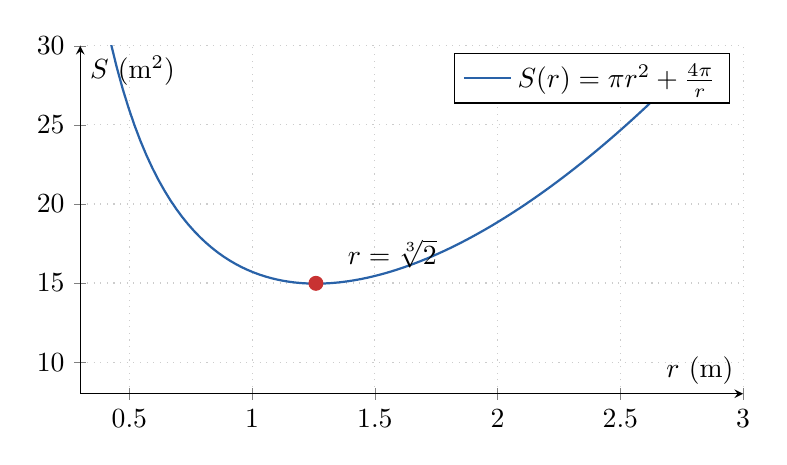
\begin{tikzpicture}
\begin{axis}[
  width=10cm, height=6cm,
  axis lines=middle,
  xlabel={$r$ (m)}, ylabel={$S$ (m$^2$)},
  xmin=0.3, xmax=3, ymin=8, ymax=30,
  grid=both,
  grid style={dotted, gray!40},
  samples=100,
]
\addplot[mainblue, thick, domain=0.4:2.8]{pi*x^2 + 4*pi/x};
\addlegendentry{$S(r) = \pi r^2 + \frac{4\pi}{r}$}
\addplot[only marks, mark=*, mark size=2.5pt, warnred] coordinates {(1.2599, 14.98)};
\node[anchor=south west] at (axis cs:1.35, 15.3) {$r = \sqrt[3]{2}$};
\end{axis}
\end{tikzpicture}
\end{center}

% ----- 应用2：物理应用 -----
\begin{appbox}[【应用2】运动学中的速度与加速度]
一质点沿直线运动，其位移函数为 $s(t) = t^3 - 6t^2 + 9t$（单位：m，$t$ 的单位：s）。求：
\begin{enumerate}[leftmargin=2em]
  \item 质点在 $t = 1$ s 时的速度和加速度；
  \item 质点何时速度为零？
  \item 质点在 $t \in [0, 4]$ 上的位移和路程。
\end{enumerate}
\end{appbox}

\textbf{解}：

(1) 速度 $v(t) = s'(t) = 3t^2 - 12t + 9$。

加速度 $a(t) = v'(t) = 6t - 12$。

$v(1) = 3 - 12 + 9 = 0$ m/s。

$a(1) = 6 - 12 = -6$ m/s\textsuperscript{2}。

(2) 令 $v(t) = 0$：$3t^2 - 12t + 9 = 0$，即 $t^2 - 4t + 3 = 0$。

$(t - 1)(t - 3) = 0$，故 $t = 1$ s 或 $t = 3$ s。

(3) 位移 $= s(4) - s(0) = (64 - 96 + 36) - 0 = 4$ m。

路程需要考虑运动方向变化。关键点：$t = 1$ 和 $t = 3$。
\begin{align*}
s(0) &= 0, \quad s(1) = 1 - 6 + 9 = 4, \\
s(3) &= 27 - 54 + 27 = 0, \quad s(4) = 4.
\end{align*}

路程 $= |s(1) - s(0)| + |s(3) - s(1)| + |s(4) - s(3)| = 4 + 4 + 4 = 12$ m。

% ----- 应用3：利润最大化 -----
\begin{appbox}[【应用3】利润最大化问题]
某企业生产一种产品，日产量为 $x$ 件时，每件成本为 $C(x) = 2x + 10 + \dfrac{50}{x}$（万元/件），产品单价为 $p = 30$（万元/件）。求日产量为多少时，日利润最大？最大日利润是多少？
\end{appbox}

\textbf{解}：日利润 = 总收入 $-$ 总成本。

总收入 $= 30x$（万元）。

总成本 $= x \cdot C(x) = x\left(2x + 10 + \dfrac{50}{x}\right) = 2x^2 + 10x + 50$（万元）。

日利润：
\[
L(x) = 30x - (2x^2 + 10x + 50) = -2x^2 + 20x - 50 \quad (x > 0)
\]

求导：$L'(x) = -4x + 20$。

令 $L'(x) = 0$，得 $x = 5$。

$L''(x) = -4 < 0$，故 $x = 5$ 为极大值点。

$L(5) = -50 + 100 - 50 = 0$（万元）。

\textbf{答}：日产量为 $5$ 件时，日利润最大，最大日利润为 $0$ 万元（即保本）。

\begin{warnbox}[注意]
本题中最大利润恰好为零，说明在给定成本结构和售价下，该产品不盈利。企业需要降低成本或提高售价才能获得正利润。这体现了导数优化在经营决策中的应用价值。
\end{warnbox}

% ============================================================
% 第四部分：课堂练习
% ============================================================
\section*{\textcolor{tipgreen}{四、课堂练习}}

\begin{enumerate}[leftmargin=2em]
  \item 求下列函数的导数：
  \begin{enumerate}[label=(\arabic*)]
    \item $f(x) = 3x^4 - 2x^3 + x - 5$
    \item $g(x) = x^2 \cos x$
    \item $h(x) = \dfrac{e^x}{x + 1}$
    \item $p(x) = \ln(x^2 + 1)$
  \end{enumerate}

  \item 求曲线 $y = \dfrac{1}{3}x^3 + x^2 - 3x + 1$ 在 $x = 1$ 处的切线方程。

  \item 求函数 $f(x) = x - \ln x$ 的单调区间和极值。

  \item 求函数 $f(x) = 2x^3 - 3x^2 - 12x + 5$ 在 $[-2, 3]$ 上的最大值和最小值。

  \item 已知 $f(x) = x^3 - \dfrac{3}{2}x^2 + a$（$a$ 为常数），若 $f(x)$ 恰好有两个零点，求 $a$ 的值。

  \item 证明：当 $x > 0$ 时，$\ln(1 + x) > x - \dfrac{x^2}{2}$。

  \item 某工厂要建造一个容积为 $750 \text{ m}^3$ 的长方体无盖蓄水池。已知池底每平方米造价为 $160$ 元，池壁每平方米造价为 $120$ 元。设水池的深为 $x$ m，底面为正方形。当 $x$ 为多少时，总造价最低？最低造价是多少？
\end{enumerate}

\vspace{10pt}

\begin{knowledgebox}[参考答案]
\textbf{1.}
\begin{enumerate}[label=(\arabic*)]
  \item $f'(x) = 12x^3 - 6x^2 + 1$
  \item $g'(x) = 2x\cos x - x^2 \sin x$
  \item $h'(x) = \dfrac{e^x(x+1) - e^x}{(x+1)^2} = \dfrac{xe^x}{(x+1)^2}$
  \item $p'(x) = \dfrac{2x}{x^2 + 1}$
\end{enumerate}

\textbf{2.} $y' = x^2 + 2x - 3$，$y'(1) = 0$，$f(1) = \frac{1}{3} + 1 - 3 + 1 = -\frac{2}{3}$。

切线方程：$y = -\dfrac{2}{3}$（水平切线）。

\textbf{3.} 定义域 $x > 0$，$f'(x) = 1 - \dfrac{1}{x} = \dfrac{x - 1}{x}$。

$f'(x) = 0$ 时 $x = 1$。$(0, 1)$ 上 $f'(x) < 0$（递减），$(1, +\infty)$ 上 $f'(x) > 0$（递增）。

$x = 1$ 处取极小值 $f(1) = 1$。无极大值。

\textbf{4.} $f'(x) = 6x^2 - 6x - 12 = 6(x-2)(x+1)$。

$f'(-1) = 0$，$f'(2) = 0$。$f(-2) = 1$，$f(-1) = 12$，$f(2) = -15$，$f(3) = -4$。

最大值 $f(-1) = 12$，最小值 $f(2) = -15$。

\textbf{5.} $f'(x) = 3x^2 - 3x = 3x(x-1)$。极大值 $f(0) = a$，极小值 $f(1) = a - \dfrac{1}{2}$。

$f(x)$ 恰有两个零点：极大值 $= 0$ 时 $a = 0$，或极小值 $= 0$ 时 $a = \dfrac{1}{2}$。

故 $a = 0$ 或 $a = \dfrac{1}{2}$。

\textbf{6.} 令 $f(x) = \ln(1+x) - x + \dfrac{x^2}{2}$（$x > 0$）。

$f'(x) = \dfrac{1}{1+x} - 1 + x = \dfrac{1 - (1+x) + x(1+x)}{1+x} = \dfrac{x^2}{1+x} > 0$。

$f(x)$ 在 $(0, +\infty)$ 上递增。$f(0) = 0$。故 $x > 0$ 时 $f(x) > 0$，即 $\ln(1+x) > x - \dfrac{x^2}{2}$。\quad $\square$

\textbf{7.} 设深为 $x$ m，底面边长为 $a$ m。$a^2 x = 750$，$a = \sqrt{\dfrac{750}{x}}$。

总造价 $P = 160a^2 + 120 \times 4ax = 160 \times \dfrac{750}{x} + 480x\sqrt{\dfrac{750}{x}} = \dfrac{120000}{x} + 480\sqrt{750x}$。

$P'(x) = -\dfrac{120000}{x^2} + \dfrac{480\sqrt{750}}{2\sqrt{x}} = -\dfrac{120000}{x^2} + \dfrac{240\sqrt{750}}{\sqrt{x}}$。

令 $P'(x) = 0$：$\dfrac{120000}{x^2} = \dfrac{240\sqrt{750}}{\sqrt{x}}$，即 $x^{3/2} = \dfrac{120000}{240\sqrt{750}} = \dfrac{500}{\sqrt{750}}$。

$x = \left(\dfrac{500}{\sqrt{750}}\right)^{2/3} = \dfrac{500^{2/3}}{750^{1/3}} = \dfrac{(500^2)^{1/3}}{750^{1/3}} = \left(\dfrac{250000}{750}\right)^{1/3} = \left(\dfrac{1000}{3}\right)^{1/3}$。

经计算 $x \approx 6.93$ m 时总造价最低。

将 $x = \sqrt[3]{\dfrac{1000}{3}}$ 代入 $P$ 计算得最低造价约为 $34641$ 元。
\end{knowledgebox}

\vfill
\begin{center}
\small\textcolor{gray}{本讲义仅供教学参考，例题可根据学生水平调整难度。}
\end{center}

\end{document}
